\begin{name}
	{\tenchude}
	{\tendethi}
	{Chuyên Hưng Yên}
	{\thoigian}
\end{name}
	\setcounter{ex}{0}\setcounter{bt}{0}
	\Opensolutionfile{ans}[ans/ans-2-GHK1-20-ChuyenHungYen-HungYen-21]

\begin{ex}%[Đề KSCL Lần 1 môn Toán THPT Chuyên Hưng Yên - Hưng Yên]%[Lê Quốc Hiệp, EX3-2021]%[2D1Y5-1]
	Bảng biến thiên sau đây là của hàm số nào?
	\begin{center}
		
\begin{tikzpicture}
			\tkzTabInit[nocadre=false,lgt=1.2,espcl=2.5,deltacl=0.6]
			{$x$ /.6,$y'$ /.6,$y$ /2}{$-\infty$,$-1$,$0$,$1$,$+\infty$}
			\tkzTabLine{,-,$0$,+,$0$,-,$0$,+,}
			\tkzTabVar{+/ $+\infty$ ,-/$-4$,+/$-3$,-/$-4$,+/$+\infty$}
		\end{tikzpicture}
	\end{center}
	\choice
	{$y=x^3-2x^2-3$}
	{$y=2x^2-3$}
	{\True $y=x^4-2x^2-3$}
	{$y=-x^4+2x^2-3$}
	\loigiai
	{
		Bảng biến thiên đã cho là của hàm số có dạng $y=ax^4+bx^2+c$ ($a\ne0$).\\
		Dựa vào bảng biến thiên suy ra $a>0$, vậy hàm số thỏa mãn là $y=x^4-2x^2-3$.
	}
\end{ex}
\begin{ex}%[Đề KSCL Lần 1 môn Toán THPT Chuyên Hưng Yên - Hưng Yên]%[Lê Quốc Hiệp, EX3-2021]%[2D2Y3-2]
	Với các số thực dương $a$, $b$ bất kì. Mệnh đề nào dưới đây đúng?
	\choice
	{$\ln\dfrac{a}{b}=\dfrac{\ln a}{\ln b}$}
	{$\ln(a+b)=\ln a\cdot\ln b$}
	{\True $\ln(ab)=\ln a+\ln b$}
	{$\ln(ab)=\ln a\cdot\ln b$}
	\loigiai
	{
		Mệnh đề đúng là $\ln(ab)=\ln a+\ln b$.
	}
\end{ex}
\begin{ex}%[Đề KSCL Lần 1 môn Toán THPT Chuyên Hưng Yên - Hưng Yên]%[Lê Quốc Hiệp, EX3-2021]%[2D1Y1-2]
	Cho hàm số $y=f(x)$ có bảng xét dấu của đạo hàm bên dưới
	\begin{center}
		
\begin{tikzpicture}
			\tkzTabInit[nocadre=false,lgt=1.2,espcl=2.5,deltacl=0.6]
			{$x$ /.6,$f'(x)$ /.8}{$-\infty$,$1$,$2$,$3$,$4$,$+\infty$}
			\tkzTabLine{,-,$0$,+,$0$,+,$0$,-,$0$,+}
		\end{tikzpicture}
	\end{center}
	Hàm số $y=f(x)$ đồng biến trên khoảng nào dưới đây?
	\choice
	{$(3;4)$}
	{$(2;4)$}
	{$(-\infty;-1)$}
	{\True $(1;3)$}
	\loigiai
	{
		Dựa vào bảng xét dấu của đạo hàm trên suy ra hàm số $y=f(x)$ đồng biến trên khoảng $(1;3)$ và $(4;+\infty)$.
	}
\end{ex}
\begin{ex}%[Đề KSCL Lần 1 môn Toán THPT Chuyên Hưng Yên - Hưng Yên]%[Lê Quốc Hiệp, EX3-2021]%[1D2Y2-1]
	Có bao nhiêu cách xếp chỗ ngồi cho $4$ bạn học sinh vào dãy có $4$ ghế?
	\choice
	{$4$}
	{$12$}
	{$8$}
	{\True $24$}
	\loigiai
	{
		Mỗi cách xếp chỗ ngồi cho $4$ bạn học sinh vào dãy có $4$ ghế là một hoán vị của $4$ phần tử.\\
		Vậy có $4!=24$ cách xếp.
	}
\end{ex}
\begin{ex}%[Đề KSCL Lần 1 môn Toán THPT Chuyên Hưng Yên - Hưng Yên]%[Lê Quốc Hiệp, EX3-2021]%[2D1Y4-1]
	Đồ thị hàm số $y=\dfrac{3x-1}{x+1}$ có đường tiệm cận ngang là
	\choice
	{$x=2$}
	{$y=-1$}
	{$x=-1$}
	{\True $y=3$}
	\loigiai
	{
		Ta có $\lim\limits_{x\to\pm\infty}y=3$ nên đồ thị hàm số đã cho có đường tiệm cận ngang là $y=3$.
	}
\end{ex}
\begin{ex}%[Đề KSCL Lần 1 môn Toán THPT Chuyên Hưng Yên - Hưng Yên]%[Lê Quốc Hiệp, EX3-2021]%[2D1Y5-4]
	\immini
	{Cho hàm số bậc ba $y=f(x)$ có đồ thị là đường cong trong hình bên. Số nghiệm thực của phương trình $f(x)=3$ là
		\choice
		{$1$}
		{$3$}
		{\True $2$}
		{$0$}}
	{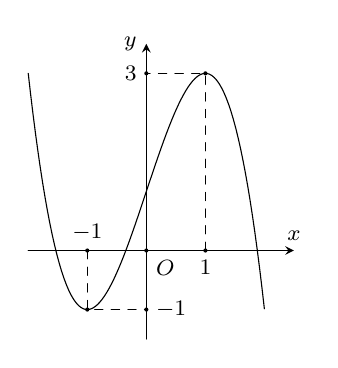
\begin{tikzpicture}[line cap=round,line join=round,font=\footnotesize,>=stealth,scale=0.75]
			\draw[->] (-2,0)--(2.5,0) node[above] {$x$};
			\draw[->] (0,-1.5)--(0,3.5) node[left] {$y$};
			\fill (0,0) circle (1pt) node [below right] {$O$}
			(-1,0) circle (1pt) node [above] {$-1$}
			(1,0) circle (1pt) node [below] {$1$}
			(0,-1) circle (1pt) node [right] {$-1$}
			(0,3) circle (1pt) node [left] {$3$}
			(1,3) circle (1pt) (-1,-1) circle (1pt);
			\draw [samples=100, domain=-2:2] plot (\x, {-(\x)^3+3*(\x)+1});
			\draw[dashed] (-1,0)|-(0,-1) (1,0)|-(0,3);
	\end{tikzpicture}}
	\loigiai
	{
		Số nghiệm thực của phương trình $f(x)=3$ bằng số giao điểm của đồ thị $y=f(x)$ và đường thẳng $y=3$.\\
		Dựa vào hình vẽ trên suy ra phương trình $f(x)=3$ có một nghiệm kép là $x=1$ và một nghiệm $x=x_0<-1$.
	}
\end{ex}
\begin{ex}%[Đề KSCL Lần 1 môn Toán THPT Chuyên Hưng Yên - Hưng Yên]%[Lê Quốc Hiệp, EX3-2021]%[2D1Y1-1]
	Trong các hàm số sau hàm nào đồng biến trên $\mathbb{R}$?
	\choice
	{$y=\dfrac{x+1}{x+3}$}
	{$y=x^2+1$}
	{$y=x^4+5x^2-1$}
	{\True $y=x^3+x$}
	\loigiai
	{
		Xét hàm số $y=x^3+x$ có tập xác định là $\mathbb{R}$ và $y'=3x^2+1>0,~\forall x\in\mathbb{R}$.\\
		Vậy $y=x^3+x$ đồng biến trên $\mathbb{R}$.
	}
\end{ex}
\begin{ex}%[Đề KSCL Lần 1 môn Toán THPT Chuyên Hưng Yên - Hưng Yên]%[Lê Quốc Hiệp, EX3-2021]%[1D3Y3-2]
	Một cấp số cộng có $u_1=-3$, $u_8=39$. Công sai của cấp số cộng đó là
	\choice
	{\True $6$}
	{$5$}
	{$8$}
	{$7$}
	\loigiai
	{
		Ta có $u_8=u_1+7d\Leftrightarrow -3+7d=39\Leftrightarrow d=6$.
	}
\end{ex}
\begin{ex}%[Đề KSCL Lần 1 môn Toán THPT Chuyên Hưng Yên - Hưng Yên]%[Lê Quốc Hiệp, EX3-2021]%[2H1Y3-2]
	Cho tứ diện $OABC$ có $OA$, $OB$, $OC$ đôi một vuông góc nhau và $OA=OB=OC=a$. Khi đó thể tích khối tứ diện $OABC$ là 
	\choice
	{$\dfrac{a^3}{2}$}
	{$\dfrac{a^3}{12}$}
	{\True $\dfrac{a^3}{6}$}
	{$\dfrac{a^3}{3}$}
	\loigiai
	{
		\immini
		{Ta có $V_{OABC}=\dfrac{1}{6}OA\cdot OB\cdot OC=\dfrac{1}{6}\cdot a^3=\dfrac{a^3}{6}$.}
		{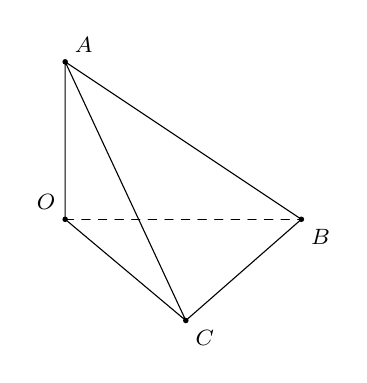
\begin{tikzpicture}[line cap=round,line join=round,font=\footnotesize,>=stealth,scale=1]
				\fill (0,0) coordinate [label=above left:$O$] (O) circle(1pt)
				(0:3) coordinate [label=below right:$B$] (B) circle(1pt)
				(90:2) coordinate [label=above right:$A$] (A) circle(1pt)
				(-40:2) coordinate [label=below right:$C$] (C) circle(1pt);
				\draw (O)--(A)--(B)--(C)--(O) (A)--(C);
				\draw[dashed] (O)--(B);
		\end{tikzpicture}}
	}
\end{ex}
\begin{ex}%[Đề KSCL Lần 1 môn Toán THPT Chuyên Hưng Yên - Hưng Yên]%[Lê Quốc Hiệp, EX3-2021]%[2H1Y3-2]
	Lăng trụ tam giác đều có độ dài tất cả các cạnh bằng $3$. Thể tích khối lăng trụ đã cho bằng
	\choice
	{$\dfrac{9\sqrt{3}}{4}$}
	{$\dfrac{9\sqrt{3}}{2}$}
	{$\dfrac{27\sqrt{3}}{2}$}
	{\True $\dfrac{27\sqrt{3}}{4}$}
	\loigiai
	{
		\immini
		{Ta có $V_{ABC.A'B'C'}=AA'\cdot S_{ABC}=3\cdot\dfrac{3^2\cdot\sqrt{3}}{4}=\dfrac{27\sqrt{3}}{4}$.}
		{\begin{tikzpicture}[line cap=round,line join=round,font=\footnotesize,>=stealth,scale=0.7]
				\fill (0,0) coordinate [label=above left:$A$] (A) circle(1pt)
				(0:4) coordinate [label=below right:$B$] (B) circle(1pt)
				(-30:3) coordinate [label=below:$C$] (C) circle(1pt)
				(90:3) coordinate [label=left:$A'$] (A') circle(1pt)
				($(A')+(B)-(A)$) coordinate [label=below right:$B'$] (B') circle(1pt)
				($(A')+(C)-(A)$) coordinate [label=below right:$C'$] (C') circle(1pt);
				\draw (A')--(A)--(C)--(B)--(B')--(C')--(A')--(B') (C)--(C');
				\draw[dashed] (A)--(B);
		\end{tikzpicture}}
	}
\end{ex}
\begin{ex}%[Đề KSCL Lần 1 môn Toán THPT Chuyên Hưng Yên - Hưng Yên]%[Lê Quốc Hiệp, EX3-2021]%[2D2Y1-2]
	Biểu thức $Q=\sqrt{a^2\cdot\sqrt[3]{a^4}}$ (với $a>0$, $a\ne1$). Đẳng thức nào sau đây là đúng?
	\choice
	{\True $Q=a^\frac{5}{3}$}
	{$Q=a^\frac{7}{4}$}
	{$Q=a^\frac{7}{3}$}
	{$Q=a^\frac{11}{6}$}
	\loigiai
	{
		Ta có $Q=\sqrt{a^2\cdot\sqrt[3]{a^4}}=\sqrt{a^2\cdot a^\frac{4}{3}}=\left(a^\frac{10}{3}\right)^\frac{1}{2}=a^\frac{5}{3}$.
	}
\end{ex}
\begin{ex}%[Đề KSCL Lần 1 môn Toán THPT Chuyên Hưng Yên - Hưng Yên]%[Lê Quốc Hiệp, EX3-2021]%[2D1Y2-1]
	Điểm cực đại của hàm số $y=x^3+3x^2+3$ là
	\choice
	{$x=0$}
	{\True $x=-2$}
	{$(0;3)$}
	{$(-2;7)$}
	\loigiai
	{
		Ta có $y'=3x^2+6x$ và $y'=0\Leftrightarrow x=0$ hoặc $x=-2$.\\
		Bảng biến thiên của hàm số $y=x^3+3x^2+3$ như sau
		\begin{center}
			
\begin{tikzpicture}
				\tkzTabInit[nocadre=false,lgt=1.2,espcl=2.5,deltacl=0.6]
				{$x$ /.6,$y'$ /.6,$y$ /2}{$-\infty$,$-2$,$0$,$+\infty$}
				\tkzTabLine{,+,$0$,-,$0$,+,}
				\tkzTabVar{-/$-\infty$ ,+/$7$,-/$3$,+/$+\infty$}
			\end{tikzpicture}
		\end{center}
		Vậy điểm cực đại của hàm số đã cho là $x=-2$.
	}
\end{ex}
\begin{ex}%[Đề KSCL Lần 1 môn Toán THPT Chuyên Hưng Yên - Hưng Yên]%[Lê Quốc Hiệp, EX3-2021]%[2D2Y3-1]
	Giá trị biểu thức $A=2^{\log_4 9+\log_2 5}$ là
	\choice
	{\True $A=15$}
	{$A=405$}
	{$A=86$}
	{$A=8$}
	\loigiai
	{
		Ta có $A=2^{\log_4 9+\log_2 5}=2^{\log_4 9}\cdot2^{\log_2 5}=3\cdot5=15$.
	}
\end{ex}
\begin{ex}%[Đề KSCL Lần 1 môn Toán THPT Chuyên Hưng Yên - Hưng Yên]%[Lê Quốc Hiệp, EX3-2021]%[2D1Y5-4]
	Số giao điểm của đường thẳng $y=4x$ và đường cong $y=x^3$ là
	\choice
	{$2$}
	{$1$}
	{$0$}
	{\True $3$}
	\loigiai
	{
		Xét phương trình hoành độ giao điểm
		\[x^3=4x\Leftrightarrow x^3-4x=0\Leftrightarrow\hoac{&x=0\\&x=\pm2.}\]
		Vậy đường thẳng $y=4x$ và đường cong $y=x^3$ có $3$ điểm chung.
	}
\end{ex}
\begin{ex}%[Đề KSCL Lần 1 môn Toán THPT Chuyên Hưng Yên - Hưng Yên]%[Lê Quốc Hiệp, EX3-2021]%[2H1Y3-2]
	Cho hình chóp $S.ABCD$ có đáy là hình vuông $ABCD$ cạnh $a$, cạnh bên $SA$ vuông góc với mặt phẳng đáy và $SA=a\sqrt{2}$. Thể tích của khối chóp $S.ABCD$ bằng
	\choice
	{$V=\sqrt{2}a^3$}
	{\True $V=\dfrac{\sqrt{2}a^3}{3}$}
	{$V=\dfrac{\sqrt{2}a^3}{6}$}
	{$V=\dfrac{\sqrt{2}a^3}{4}$}
	\loigiai
	{
		\immini
		{Ta có $V_{ABCD}=\dfrac{1}{3}SA\cdot S_{ABCD}=\dfrac{1}{3}\cdot a\sqrt{2}\cdot a^2=\dfrac{a^3\sqrt{2}}{3}$.}
		{\begin{tikzpicture}[line cap=round,line join=round,font=\footnotesize,>=stealth,scale=0.75]
				\fill (0,0) coordinate [label=above left:$A$] (A) circle(1pt)
				(0:3) coordinate [label=below right:$B$] (B) circle(1pt)
				(90:2) coordinate [label=above right:$S$] (S) circle(1pt)
				(-40:2) coordinate [label=below right:$C$] (C) circle(1pt)
				($(A)+(C)-(B)$) coordinate [label=below:$D$] (D) circle(1pt);
				\draw (S)--(B)--(C) (D)--(S)--(C)--(D);
				\draw[dashed] (D)--(A)--(S) (A)--(B);
		\end{tikzpicture}}
	}
\end{ex}
\begin{ex}%[Đề Khảo sát chất lượng Chuyên Hưng Yên 2020-2021]%[Nguyễn Tấn Linh, dự án 12-EX-3-2021]%[2H1Y1-2]
	Hình lăng trụ tam giác có bao nhiêu mặt?
	\choice
	{$6$}
	{$4$}
	{\True $5$}
	{$3$}
	\loigiai{}
\end{ex}
\begin{ex}%[Đề Khảo sát chất lượng Chuyên Hưng Yên 2020-2021]%[Nguyễn Tấn Linh, dự án 12-EX-3-2021]%[2D1Y2-2]
	Cho hàm số $y=f(x)$ có bảng biến thiên như sau
	\begin{center}
		
\begin{tikzpicture}[>=stealth]
			\tkzTabInit[nocadre=false,lgt=1,espcl=2,deltacl=0.5]{$x$/.7 ,$y'$/.7,$y$/2}
			{$-\infty$ , $-1$ , $0$ , $1$ , $+\infty$}
			\tkzTabLine{ , - , $0$ , + , $0$ , - , $0$ , + ,}
			\tkzTabVar{+/$+\infty$ , -/$0$, +/$3$ , -/$0$ , +/$+\infty$}
		\end{tikzpicture}
	\end{center}
	Khẳng định nào sau đây \textbf{sai}?
	\choice
	{Hàm số có ba điểm cực trị}
	{\True Hàm số đạt cực đại tại điểm $x=3$}
	{Hàm số có hai điểm cực tiểu}
	{Hàm số đạt cực đại tại điểm $x=0$}
	\loigiai{Dựa vào bảng biến thiên, ta thấy hàm số đạt cực đại tại $x=0$.}
\end{ex}
\begin{ex}%[Đề Khảo sát chất lượng Chuyên Hưng Yên 2020-2021]%[Nguyễn Tấn Linh, dự án 12-EX-3-2021]%[1D5Y2-2]
	Cho hàm số $y=x^3-x-1$ có đồ thị $\left(C\right)$. Phương trình tiếp tuyến của $\left(C\right)$ tại giao điểm của
	$\left(C\right)$ với trục tung là
	\choice
	{$y=2x-1$}
	{$y=2x+2$}
	{$y=-x+1$}
	{\True $y=-x-1$}
	\loigiai{
		Đạo hàm $y'=3x^2-1$.\\
		Giao điểm của $\left(C\right)$ với trục tung là $A\left(0;-1\right)$.\\
		Phương trình tiếp tuyến của $\left(C\right)$ tại $A\left(0;-1\right)$ là $y=y'\left(0\right)\left(x-0\right)-1\Leftrightarrow y=-x-1$.
	}
\end{ex}
\begin{ex}%[Đề Khảo sát chất lượng Chuyên Hưng Yên 2020-2021]%[Nguyễn Tấn Linh, dự án 12-EX-3-2021]%[2D1Y5-3]
	Cho hàm số $y=f(x)$ có bảng biến thiên
	\begin{center}
		
\begin{tikzpicture}[>=stealth]
			\tkzTabInit[nocadre=false,lgt=1,espcl=2,deltacl=0.5]{$x$/.7 ,$y'$/.7,$y$/2}
			{$-\infty$ , $-1$ , $1$ , $+\infty$}
			\tkzTabLine{ , - , $0$ , + , $0$ , - ,}
			\tkzTabVar{+/$+\infty$ , -/$-4$ , +/$0$ , -/$-\infty$}
		\end{tikzpicture}
	\end{center}
	Với giá trị nào của $m$ thì phương trình $f(x)+m=0$ có $3$ nghiệm phân biệt?
	\choice
	{$-1<m<1$}
	{$-4<m<0$}
	{\True $0<m<4$}
	{$-2<m<1$}
	\loigiai{Phương trình $f(x)+m=0\Leftrightarrow f(x)=-m$.\\
		Dựa vào bảng biến thiên ta có $-4<-m<0\Leftrightarrow 0<m<4$.
	}
\end{ex}
\begin{ex}%[Đề Khảo sát chất lượng Chuyên Hưng Yên 2020-2021]%[Nguyễn Tấn Linh, dự án 12-EX-3-2021]%[2D1Y5-1]
	\immini
	{
		Đường cong ở hình bên là đồ thị của hàm số $y=\dfrac{ax+b}{cx+d}$ với $a,b,c,d$ là các số thực. Mệnh đề nào sau đây đúng?
		\choice
		{$y'>0,\forall x\ne 1$}
		{\True $y'<0,\forall x\in \mathbb{R}$}
		{$y'<0,\forall x\ne 1$}
		{$y'>0,\forall x\in \mathbb{R}$}
	}
	{
		\begin{tikzpicture}[line join = round, line cap = round,>=stealth,font=\footnotesize,scale=0.4]
			\def\xt{-5} \def\xp{6} \def\yd{-5} \def\yt{5}
			\def\a{1} 
			\def\b{1}
			\def\c{1}
			\def\d{-1}
			\draw[->] (\xt,0)--(\xp,0) node[below]{$x$};
			\draw[->] (0,\yd)--(0,\yt) node[left]{$y$};
			\fill (0,0) circle (1.5pt) node[above right=-2pt]{$O$};
			\fill (1,0) circle (1.5pt) node[below right]{$1$};
			\begin{scope}
				\clip (\xt+0.1,\yd+0.1) rectangle (\xp-0.1,\yt-0.1);
				\pgfmathsetmacro{\tcn}{(\a)/(\c)}
				\pgfmathsetmacro{\tcd}{-(\d)/(\c)}
				\draw[dashed] (\xt,\tcn)--(\xp,\tcn) (\tcd,\yd)--(\tcd,\yt);
				\draw[samples=150,smooth,domain={\tcd+0.01}:\xp] plot(\x,{(\a*\x+(\b))/(\c*\x+(\d))});
				\draw[samples=150,smooth,domain=\xt:{\tcd-0.01}] plot(\x,{(\a*\x+(\b))/(\c*\x+(\d))});
			\end{scope}
		\end{tikzpicture}
	}
	\loigiai{Dựa vào đồ thị ta thấy hàm số có tập xác định là $\mathscr{D}=\mathbb{R}\setminus \left\{1 \right\}$, hàm số luôn nghịch biến trên khoảng $\left(-\infty;1\right)$, $\left(1;+\infty\right)$ nên $y'<0,\forall x\ne 1$.
	}
\end{ex}
\begin{ex}%[Đề Khảo sát chất lượng Chuyên Hưng Yên 2020-2021]%[Nguyễn Tấn Linh, dự án 12-EX-3-2021]%[2D1Y1-1]
	Hàm số $y=3x^4+2$ nghịch biến trên khoảng nào sau đây?
	\choice
	{\True $\left(-\infty;0\right)$}
	{$\left(0;+\infty\right)$}
	{$\left(-\dfrac{2}{3};+\infty\right)$}
	{$\left(-\infty;\dfrac{2}{3}\right)$}
	\loigiai{Ta có $y'=12x^3$.\\
		Xét bất phương trình $y'< 0\Leftrightarrow 12x^3< 0\Leftrightarrow x<0$.\\
		Vậy hàm số nghịch biến trên $\left(-\infty;0\right)$.
	}
\end{ex}
\begin{ex}%[Đề Khảo sát chất lượng Chuyên Hưng Yên 2020-2021]%[Nguyễn Tấn Linh, dự án 12-EX-3-2021]%[2D2Y1-1]
	Giá trị của biểu thức $P=\dfrac{2^{3}\cdot2^{-1}+5^{-3}\cdot5^{4}}{10^{-3}:10^{-2}-\left(0,1\right)^0}$ là
	\choice
	{$10$}
	{$9$}
	{\True $-10$}
	{$-9$}
	\loigiai{Ta có $P=\dfrac{2^{3}\cdot2^{-1}+5^{-3}\cdot5^{4}}{10^{-3}:10^{-2}-\left(0,1\right)^0}=\dfrac{2^{2}+5}{10^{-1}-1}=\dfrac{4+5}{\dfrac{1}{10}-1}=-10$.
	}
\end{ex}
\begin{ex}%[Đề Khảo sát chất lượng Chuyên Hưng Yên 2020-2021]%[Nguyễn Tấn Linh, dự án 12-EX-3-2021]%[2D1Y4-1]
	Đồ thị hàm số $y=\dfrac{x+1}{x^2+2x-3}$ có bao nhiêu đường tiệm cận?
	\choice
	{$2$}
	{$0$}
	{$1$}
	{\True $3$}
	\loigiai{Tập xác định $\mathscr{D}=\mathbb{R}\setminus\left\{1;-3 \right\}$.\\
		Ta có $\lim\limits_{x\to \pm \infty}y=\lim\limits_{x\to \pm \infty}\dfrac{x+1}{x^2+2x-3}=0$. Vậy $y=0$ là tiệm cận ngang của đồ thị hàm số.\\
		$\lim\limits_{x\to \left(-3\right)^{+}}y=\lim\limits_{x\to \left(-3\right)^{+}}\dfrac{x+1}{x^2+2x-3}=+\infty$ và $\lim\limits_{x\to 1^{+}}y=\lim\limits_{x\to 1^{+}}\dfrac{x+1}{x^2+2x-3}=+\infty$.\\
		Vậy $x=1$; $x=-3$ là các đường tiệm cận đứng của đồ thị hàm số.
	}
\end{ex}
\begin{ex}%[Đề Khảo sát chất lượng Chuyên Hưng Yên 2020-2021]%[Nguyễn Tấn Linh, dự án 12-EX-3-2021]%[2H1Y2-2]
	Số cạnh của hình mười hai mặt đều là
	\choice
	{$16$}
	{$12$}
	{$20$}
	{\True $30$}
	\loigiai{
		\immini
		{
			Đa diện mười hai mặt đều là đa diện đều loại $\left\{5;3 \right\}$ có $30$ cạnh.
		}
		{
			\begin{tikzpicture}[line join=round,line cap=round,font=\footnotesize,scale=0.7]
				\foreach \x in {0,1,2,...,9}{
					\coordinate (A\x) at (36+\x*36:3);
					\coordinate (B\x) at ($(0,0)!.7!(A\x)$);}
				\foreach[evaluate=\i as \ki using {int(mod(\i+1,10))}] \i in {0,...,9}
				\draw (A\i) to (A\ki);
				\foreach \i in {1,3,5,7,9}
				\draw (B\i)--(A\i);
				\draw (B1)--(B3)--(B5)--(B7)--(B9)--cycle;
				\foreach \i in {0,2,4,6,8}
				\draw[dashed] (B\i)--(A\i);
				\draw[dashed] (B2)--(B4)--(B6)--(B8)--(B0)--cycle;
			\end{tikzpicture}
		}
	}
\end{ex}
\begin{ex}%[Đề Khảo sát chất lượng Chuyên Hưng Yên 2020-2021]%[Nguyễn Tấn Linh, dự án 12-EX-3-2021]%[2H1Y3-2]
	Cho khối lăng trụ có diện tích đáy $B=3$ và chiều cao $h=2$. Thể tích khối lăng trụ đã cho bằng
	\choice
	{$3$}
	{$12$}
	{$2$}
	{\True $6$}
	\loigiai{Thể tích khối lăng trụ đã cho bằng $V=Bh=3\cdot2=6$. 
	}
\end{ex}
\begin{ex}%[Đề KSCL Lần 1 môn Toán THPT Chuyên Hưng Yên - Hưng Yên]%[Lê Quốc Hiệp, EX3-2021]%[2H1B2-3]
	Hình chóp tứ giác đều có bao nhiêu mặt phẳng đối xứng?
	\choice
	{$2$}
	{$1$}
	{\True $4$}
	{$3$}
	\loigiai
	{
		\immini
		{Hình chóp tứ giác đều $S.ABCD$ có $4$ mặt phẳng đối xứng gồm: $(SAC)$, $(SBD)$, mặt phẳng trung trực của cạnh $BC$ và mặt phẳng trung trực của cạnh $AB$.}
		{\begin{tikzpicture}[line cap=round,line join=round,font=\footnotesize,>=stealth,scale=1]
				\fill (0,0) coordinate [label=below:$A$] (A) circle(1pt)
				(0:3) coordinate [label=below right:$B$] (B) circle(1pt)
				(70:2) coordinate [label=above right:$S$] (S) circle(1pt)
				(-40:2) coordinate [label=below right:$C$] (C) circle(1pt)
				($(A)+(C)-(B)$) coordinate [label=below:$D$] (D) circle(1pt);
				\draw ($0.5*(B)+0.5*(C)$)--(S)--(B)--(C) (D)--(S)--(C)--(D);
				\draw[dashed] (D)--(A)--(S)--($0.5*(A)+0.5*(B)$) (C)--(A)--(B)--(D) ($0.5*(B)$)--($0.5*(D)+0.5*(C)$)--(S)--($0.5*(D)$)--($0.5*(B)+0.5*(C)$);
		\end{tikzpicture}}
	}
\end{ex}
\begin{ex}%[Đề KSCL Lần 1 môn Toán THPT Chuyên Hưng Yên - Hưng Yên]%[Lê Quốc Hiệp, EX3-2021]%[2H1B3-2]
	Cho hình lăng trụ tam giác đều $ABC.A'B'C'$ có $AB=a$, góc giữa đường thẳng $A'C$ và mặt phẳng $(ABC)$ bằng $45^\circ$. Thể tích khối lăng trụ $ABC.A'B'C'$ bằng
	\choice
	{$\dfrac{a^3\sqrt{3}}{12}$}
	{\True $\dfrac{a^3\sqrt{3}}{4}$}
	{$\dfrac{a^3\sqrt{3}}{2}$}
	{$\dfrac{a^3\sqrt{3}}{6}$}
	\loigiai
	{
		\immini
		{Hình chiếu vuông góc của $A'C$ lên mặt phẳng $(ABC)$ là $AC$.
			Suy ra $\widehat{A'CA}=45^\circ$.\\
			Khi đó tam giác $A'AC$ vuông cân tại $A$ và $AA'=AC=AB=a$.\\
			Ta có $V_{ABC.A'B'C'}=AA'\cdot S_{ABC}=a\cdot\dfrac{a^2\sqrt{3}}{4}=\dfrac{a^3\sqrt{3}}{4}$.
		}
		{\begin{tikzpicture}[line cap=round,line join=round,font=\footnotesize,>=stealth,scale=0.75]
				\fill (0,0) coordinate [label=above left:$A$] (A) circle(1pt)
				(0:4) coordinate [label=below right:$B$] (B) circle(1pt)
				(-30:3) coordinate [label=below:$C$] (C) circle(1pt)
				(90:3) coordinate [label=left:$A'$] (A') circle(1pt)
				($(A')+(B)-(A)$) coordinate [label=below right:$B'$] (B') circle(1pt)
				($(A')+(C)-(A)$) coordinate [label=below right:$C'$] (C') circle(1pt);
				\draw (A')--(A)--(C)--(B)--(B')--(C')--(A')--(B') (A')--(C)--(C');
				\draw[dashed] (A)--(B);
				\tkzMarkAngle[size=.6cm](A',C,A)
		\end{tikzpicture}}
	}
\end{ex}
\begin{ex}%[Đề KSCL Lần 1 môn Toán THPT Chuyên Hưng Yên - Hưng Yên]%[Lê Quốc Hiệp, EX3-2021]%[2D1B2-1]
	Cho hàm số $f(x)$ có đạo hàm $f'(x)=x(x^3-x)(x+1)^2$ với mọi $x$ thuộc $\mathbb{R}$. Số điểm cực trị của hàm số $f(x)$ là
	\choice
	{$0$}
	{\True $2$}
	{$3$}
	{$1$}
	\loigiai
	{
		Ta có $f'(x)=0\Leftrightarrow\hoac{&x=0\\&x^3-x=0\\&(x+1)^2=0}\Leftrightarrow \hoac{&x=0\\&x=\pm1.}$\\
		Bảng xét dấu của $f'(x)$ như bên dưới
		\begin{center}
			
\begin{tikzpicture}
				\tkzTabInit[nocadre=false,lgt=1.2,espcl=2.5,deltacl=0.6]
				{$x$ /.6,$f'(x)$ /.8}{$-\infty$,$-1$,$0$,$1$,$+\infty$}
				\tkzTabLine{,+,$0$,-,$0$,-,$0$,+}
			\end{tikzpicture}
		\end{center}
		Vậy hàm số đã cho có $2$ điểm cực trị là $x=\pm1$.
	}
\end{ex}
\begin{ex}%[Đề KSCL Lần 1 môn Toán THPT Chuyên Hưng Yên - Hưng Yên]%[Lê Quốc Hiệp, EX3-2021]%[1H3B5-4]
	Cho hình chóp $S.ABCD$ có đáy là hình vuông $ABCD$ cạnh $a$, cạnh bên $SA$ vuông góc với mặt phẳng đáy và $SA=a$. Tính khoảng cách giữa hai đường thẳng $SA$ và $CD$.
	\choice
	{$\dfrac{a\sqrt{2}}{2}$}
	{$a\sqrt{2}$}
	{\True $a$}
	{$2a$}
	\loigiai
	{
		\immini
		{Ta có $\heva{&AD\perp SA\\&AD\perp CD}\Rightarrow AD$ là đoạn vuông góc chung của $SA$ và $CD$.\\
			Vậy khoảng cách giữa hai đường thẳng $SA$ và $CD$ bằng $AD=a$.	
		}
		{\begin{tikzpicture}[line cap=round,line join=round,font=\footnotesize,>=stealth,scale=0.75]
				\fill (0,0) coordinate [label=above left:$A$] (A) circle(1pt)
				(0:3) coordinate [label=below right:$B$] (B) circle(1pt)
				(90:2) coordinate [label=above right:$S$] (S) circle(1pt)
				(-40:2) coordinate [label=below right:$C$] (C) circle(1pt)
				($(A)+(C)-(B)$) coordinate [label=below:$D$] (D) circle(1pt);
				\draw (S)--(B)--(C) (D)--(S)--(C)--(D);
				\draw[dashed] (D)--(A)--(S) (A)--(B);
		\end{tikzpicture}}
	}
\end{ex}
\begin{ex}%[Đề KSCL Lần 1 môn Toán THPT Chuyên Hưng Yên - Hưng Yên]%[Lê Quốc Hiệp, EX3-2021]%[2H1B3-2]
	Cho hình chóp $S.ABC$ có đáy $ABC$ là tam giác vuông cân tại $B$ và $AB=2a$. Tam giác $SAB$ đều và nằm trong mặt phẳng vuông góc với đáy. Tính thể tích $V$ của khối chóp $S.ABC$
	\choice
	{$V=\dfrac{a^3\sqrt{3}}{4}$}
	{\True $V=\dfrac{a^3\sqrt{3}}{3}$}
	{$V=\dfrac{a^3\sqrt{3}}{12}$}
	{$V=\dfrac{2a^3\sqrt{3}}{3}$}
	\loigiai
	{
		\immini
		{
			Gọi $H$ là trung điểm của $AB\Rightarrow SH\perp AB$. Khi đó $SH\perp(ABC)$.\\
			Ta có $S_{ABC}=\dfrac{AB^2}{2}=\dfrac{4a^2}{2}=2a^2$.\\
			Vậy $V_{S.ABC}=\dfrac{1}{3}SH\cdot S_{ABC}=\dfrac{1}{3}\cdot\dfrac{a\sqrt{3}}{2}\cdot2a^2=\dfrac{a^3\sqrt{3}}{3}$.
		}
		{\begin{tikzpicture}[line cap=round,line join=round,font=\footnotesize,>=stealth,scale=1]
				\fill (0,0) coordinate [label=above left:$A$] (A) circle(1pt)
				(0:3) coordinate [label=below right:$C$] (C) circle(1pt)
				(70:2) coordinate [label=above right:$S$] (S) circle(1pt)
				(-40:2) coordinate [label=below right:$B$] (B) circle(1pt)
				($(A)!0.5!(B)$) coordinate [label=below:$H$] (H) circle(1pt);
				\draw (A)--(S)--(C)--(B)--(A) (H)--(S)--(B);
				\draw[dashed] (A)--(C);
				\tkzMarkRightAngles[size=0.2](A,B,C)
		\end{tikzpicture}}
	}
\end{ex}
\begin{ex}%[Đề Khảo sát chất lượng Chuyên Hưng Yên 2020-2021]%[Nguyễn Tấn Linh, dự án 12-EX-3-2021]%[2D2B3-2]
	Biết $\log_ab=2$; $\log_ac=3$; $a,b,c>0$; $a\ne 1$. Khi đó giá trị của $\log_a\left(\dfrac{a^2\sqrt[3]{b}}{c}\right)$ bằng
	\choice
	{$6$}
	{$\dfrac{2}{3}$}
	{$5$}
	{\True $-\dfrac{1}{3}$}
	\loigiai{$\log_a\left(\dfrac{a^2\sqrt[3]{b}}{c}\right)=\log_aa^2+\log_a\sqrt[3]{b}-\log_ac=2\log_aa+\dfrac{1}{3}\log_ab-\log_ac=2+\dfrac{1}{3}\cdot2-3=-\dfrac{1}{3}$.
	}
\end{ex}
\begin{ex}%[Đề Khảo sát chất lượng Chuyên Hưng Yên 2020-2021]%[Nguyễn Tấn Linh, dự án 12-EX-3-2021]%[2D1B3-1]
	Giá trị lớn nhất của hàm số $y=2x^3+3x^2-12x+2$ trên đoạn $\left[-1;2 \right]$ là
	\choice
	{$6$}
	{$11$}
	{\True $15$}
	{$10$}
	\loigiai{Hàm số xác định và liên tục trên đoạn $\left[-1;2 \right]$.\\
		Ta có $y'=6x^2+6x-12$. $y'=0\Leftrightarrow \hoac{& x=-2\notin \left[-1;2 \right] \\& x=1\in \left[-1;2 \right].}$\\
		Ta tính $y\left(-1\right)=15;y\left(2\right)=6;y\left(1\right)=-5$.\\
		Vậy giá trị lớn nhất của hàm số là $15$.
	}
\end{ex}
\begin{ex}%[Đề Khảo sát chất lượng Chuyên Hưng Yên 2020-2021]%[Nguyễn Tấn Linh, dự án 12-EX-3-2021]%[2D2B1-1]
	Biết $9^x+9^{-x}=23$. Tính giá trị của biểu thức $P=3^x+3^{-x}$.
	\choice
	{$25$}
	{$\sqrt{27}$}
	{$\sqrt{23}$}
	{\True $5$}
	\loigiai{$P=3^x+3^{-x}\Leftrightarrow P^2=9^x+9^{-x}+2=25\Rightarrow P=5$.
	}
\end{ex}
\begin{ex}%[Đề Khảo sát chất lượng Chuyên Hưng Yên 2020-2021]%[Nguyễn Tấn Linh, dự án 12-EX-3-2021]%[2D1B5-6]
	Có bao nhiêu tiếp tuyến của đồ thị hàm số $y=x^3+3x^2-3$ song song với trục hoành?
	\choice
	{$0$}
	{\True $2$}
	{$1$}
	{$3$}
	\loigiai{Ta có $y'=3x^2+6x$, $y'=0\Leftrightarrow \hoac{& x=0\Rightarrow y=-3 \\& x=-2\Rightarrow y=1.}$\\
		Tại điểm cực trị thì tiếp tuyến có hệ số góc bằng $0$ và nếu tung độ là số khác $0$ thì tiếp tuyến tại điểm cực trị của đồ thị song song với trục hoành.\\
		Vậy có $2$ tiếp tuyến song song với trục hoành.
	}
\end{ex}
\begin{ex}%[Đề Khảo sát chất lượng Chuyên Hưng Yên 2020-2021]%[Nguyễn Tấn Linh, dự án 12-EX-3-2021]%[1H3B3-3]
	Cho hình chóp $S.ABC$ có đáy là tam giác đều cạnh $a$, $SA$ vuông góc với mặt phẳng đáy và $SA=a$. Góc giữa $SB$ và mặt phẳng đáy bằng
	\choice
	{\True $45^\circ$}
	{$60^\circ$}
	{$30^\circ$}
	{$90^\circ$}
	\loigiai{
		\immini
		{
			Ta có $SA\perp \left(ABC\right)\Rightarrow \widehat{\left(SB,\left(ABC\right)\right)}=\widehat{SBA}$.\\
			Trong tam giác vuông $SAB$ ta có $$\tan \widehat{SBA}=\dfrac{SA}{AB}=1\Rightarrow \widehat{SBA}=45^\circ.$$ Vậy $\widehat{\left(SB,\left(ABC\right)\right)}=45^\circ$.
		}
		{
			\begin{tikzpicture}[line join=round,line cap=round,font=\footnotesize,scale=1]
				\coordinate[label=left:$A$] (A) at (0,0);
				\coordinate[label=below left:$B$] (B) at (1,-1);
				\coordinate[label=right:$C$] (C) at (4,0);
				\coordinate[label=above left:$S$] (S) at ($(A)+(90:3)$);
				\tkzMarkAngles[size=0.7](S,B,A)
				\draw (A)--(B)--(C)--(S)--cycle (S)--(B);
				\draw[dashed] (A)--(C);
				\draw ($ (A)!5pt!(C)$)--($(A)!2!($($(A)!5pt!(C)$)!.5!($(A)!5pt!(S)$)$)$)--($(A)!5pt!(S)$);
				\foreach \diem in {A,B,C,S} \fill (\diem) circle(1.5pt);
			\end{tikzpicture}
		}
	}
\end{ex}
\begin{ex}%[Đề Khảo sát chất lượng Chuyên Hưng Yên 2020-2021]%[Nguyễn Tấn Linh, dự án 12-EX-3-2021]%[2D1K1-3]
	Gọi $S$ là tập hợp các giá trị nguyên dương của $m$ để hàm số $y=x^3-3\left(2m+1\right)x^2+\left(12m+5\right)x+2$ đồng biến trên khoảng $\left(2;+\infty\right)$. Số phần tử của $S$ bằng
	\choice
	{$2$}
	{$3$}
	{\True $0$}
	{$1$}
	\loigiai{Ta có $y'=3x^2-6\left(2m+1\right)x+12m+5$.\\
		Hàm số đồng biến khoảng $\left(2;+\infty\right)$
		\allowdisplaybreaks
		\begin{eqnarray*}
			&\Leftrightarrow& y'\ge 0,\forall x\in \left(2;+\infty\right)\\
			&\Leftrightarrow& 3x^2-6\left(2m+1\right)x+12m+5\ge 0\,\forall x\in \left(2;+\infty\right)\\
			&\Leftrightarrow& 3x^2-6x+5\ge 12m\left(x-1\right)\\
			&\Leftrightarrow& \dfrac{3x^2-6x+5}{x-1}\ge 12m.
		\end{eqnarray*}
		Xét hàm số $f(x)=\dfrac{3x^2-6x+5}{x-1}$; $f'(x)=\dfrac{3x^2-6x+1}{\left(x-1\right)^{2}}=3-\dfrac{2}{\left(x-1\right)^{2}}>0,\forall x>2$.\\
		Suy ra hàm số $f(x)$ đồng biến trên khoảng $\left(2;+\infty\right)$.\\
		Do đó $f(x)>f\left(2\right),\forall x\in \left(2;+\infty\right)\Rightarrow 12m\le f\left(2\right)=5\Rightarrow m\le \dfrac{5}{12}$.\\
		Vì $m$ nguyên dương suy ra không tồn tại $m$ thỏa mãn bài toán.
	}
\end{ex}
\begin{ex}%[Đề Khảo sát chất lượng Chuyên Hưng Yên 2020-2021]%[Nguyễn Tấn Linh, dự án 12-EX-3-2021]%[2D1K3-6]
	Một loại thuốc được dùng cho một bệnh nhân và nồng độ thuốc trong máu của bệnh nhân được giám sát bởi bác sĩ. Biết rằng nồng độ thuốc trong máu của bệnh nhân sau khi tiêm vào cơ thể trong $t$ giờ được cho bởi công thức $c(t)=\dfrac{t}{t^2+1}$ (mg/L). Sau khi tiêm thuốc bao lâu thì nồng độ thuốc trong máu của bệnh nhân cao nhất?
	\choice
	{$4$ giờ}
	{$3$ giờ}
	{\True $1$ giờ}
	{$2$ giờ}
	\loigiai{Ta có $c'(t)=\dfrac{-t^2+1}{\left(t^2+1\right)^{2}},\forall t\in \left(0;+\infty\right)$. Cho $c'(t)=0\Leftrightarrow \hoac{& t=1 \\& t=-1\,\, \text{(loại)}.}$\\
		Bảng biến thiên
		\begin{center}
			
\begin{tikzpicture}[>=stealth]
				\tkzTabInit[nocadre=false,lgt=1.3,espcl=2,deltacl=0.5]{$t$/.7 ,$c'(t)$/.7,$c(t)$/2}
				{$0$ , $1$ , $+\infty$}
				\tkzTabLine{ , + , $0$ , - ,}
				\tkzTabVar{-/ , +/ , -/}
			\end{tikzpicture}
		\end{center}
		Vậy sau khi tiêm $1$ giờ, nồng độ thuốc trong máu bệnh nhân cao nhất.
	}
\end{ex}
\begin{ex}%[THPT Chuyên Hưng Yên, 2020-2021]%[Nguyễn Xuân Bảo, 12-EX3-2021]%[2D1K5-1]
	\immini
	{Cho hàm số $y=a{x^3}+b{x^2}+cx+d$ $(a,b,c,d \in \mathbb{R})$ có đồ thị là đường cong trong hình bên. 
		Có bao nhiêu số dương trong các số $a$ , $b$ , $c$ , $d$ ?
		\choice
		{$4$}
		{$1$}
		{\True $2$}
		{$3$}}
	{\begin{tikzpicture}[scale=0.8, font=\footnotesize, line join=round, line cap=round, >=stealth]
			\def\a{-0.3987}
			\def\b{2.446}
			\def\c{-3.1144}
			\def\d{0.3174}
			\draw (0,0) node [below left] {$O$};
			\draw[->] (-1,0)--(5,0) node[below] {$x$};
			\draw[->] (0,-1)--(0,3.5) node[below left] {$y$};
			\draw[samples=200,domain=-0.57:4.59,smooth,variable=\x] plot (\x,{\a*(\x)^3+\b*(\x)^2+\c*(\x)+\d});
	\end{tikzpicture}}
	
	\loigiai{
		Ta có $\lim\limits_{x\to+\infty}y=-\infty $$\Rightarrow $ $a < 0$ .\\
		Gọi $x_1$, $x_2$ là hoành độ hai điểm cực trị của hàm số suy ra $x_1$, $x_2$ nghiệm phương trình $ y'=3a{x^2}+2bx+c=0$ nên theo định lý Vi-ét
		\begin{itemize}
			\item Tổng hai nghiệm $x_1+x_2=-\dfrac{2b}{3a}> 0$ $\Rightarrow $ $\dfrac{b}{a}< 0$ $\Rightarrow $ $b > 0$ .
			\item Tích hai nghiệm $x_1x_2=\dfrac{c}{3a}> 0$ $\Rightarrow $ $c < 0$.
		\end{itemize}
		Lại có đồ thị hàm số cắt trục tung tại điểm có tung độ dương nên $d > 0$ .\\
		Vậy có $2$ số dương trong các số $a$ , $b$ , $c$ , $d$.}
\end{ex}
\begin{ex}%[THPT Chuyên Hưng Yên, 2020-2021]%[Nguyễn Xuân Bảo, 12-EX3-2021]%[2D1K2-5]
	Tìm các giá trị của tham số $m$ để đồ thị hàm số  $y=m{x^4}+(2m-1){x^2}+m-2$ $(a,b,c,d \in \mathbb{R})$ chỉ có một điểm cực đại và không có điểm cực tiểu.
	\choice
	{$\hoac{& m \le 0\\ & m > \dfrac{1}{2}}$}
	{\True $m \le 0$}
	{ $\hoac{& m \le 0\\ & m \ge \dfrac{1}{2}}$}
	{$m \le \dfrac{1}{2}$}
	\loigiai{
		\begin{itemize}
			\item Trường hợp $1$. Xét $m=0$, hàm số trở thành $y=-x^2-2$. Khi đó đồ thị hàm số chỉ có một điểm cực đại và không có điểm cực tiểu, nhận $m=0$.
			\item Trường hợp 2. Xét $m \ne 0$.\\
			Đồ thị hàm số chỉ có một điểm cực đại và không có điểm cực tiểu \[\Leftrightarrow \heva{&a<0\\&ab \ge 0} \Leftrightarrow \heva{&m<0\\&m (2m-1) \ge 0} \Leftrightarrow \heva{&m<0\\& \hoac{& m \le 0\\ & m \ge \dfrac{1}{2}}} \Leftrightarrow  m < 0.\]
		\end{itemize}	
		Kết luận. Từ trường hợp $1$ và $2$ ta có $ m \le 0$.
	}
\end{ex}
\begin{ex}%[THPT Chuyên Hưng Yên, 2020-2021]%[Nguyễn Xuân Bảo, 12-EX3-2021]%[2D1K5-4]
	Tìm tất cả các giá trị của tham số $m$ để đường thẳng $(d) \colon y=x+m-1$ cắt đồ thị hàm số $y= \dfrac{2x+1}{x+1}$ tại hai điểm phân biệt $M$, $N$ sao cho $MN=2 \sqrt {3}$.
	\choice
	{ $\hoac{& m= 2+\sqrt{10}\\ & m = 2-\sqrt{10}}$}
	{$\hoac{& m= 4+\sqrt{3}\\ & m = 4-\sqrt{3}}$}
	{$\hoac{& m= 2+\sqrt{3}\\ & m = 2-\sqrt{3}}$}
	{\True $\hoac{& m= 4 +\sqrt{10}\\ & m = 4-\sqrt{10}}$}
	\loigiai{
		Phương trình hoành độ giao điểm, với $x \ne -1$, ta có 
		\[x+m-1= \dfrac{2x+1}{x+1}, x \ne -1.\] 
		Vì $x=-1$ không là nghiệm nên phương trình được biến đổi thành
		\[ x^2+(m-2)x+m-2=0 \,\, (1) . \]
		$(d)$ cắt $(C)$ tại hai điểm phân biệt $\Leftrightarrow$ $(1)$ có hai nghiệm phân biệt $\Leftrightarrow \Delta >0 \Leftrightarrow \hoac{&m<2\\&m>6.}$\\
		Giả sử $M(x_1;x_1+m-1)$, $N(x_2;x_2+m-1)$, trong đó $x_1$, $x_2$ là nghiệm của phương trình $(1)$ và $x_1+x_2=2-m$, $x_1x_2=m-2$.\\
		Ta có
		\begin{align*}
			MN=2\sqrt{3} & \Leftrightarrow  \sqrt{(x_2-x_1)^2+(x_2-x_1)^2}=2\sqrt3  \Leftrightarrow 2(x_1^2+x_2^2-2x_1x_2)=12\\ &  \Leftrightarrow (x_1+x_2)^2-4x_1x_2=6 \Leftrightarrow (2-m)^2-4(m-2)-6=0
			\Leftrightarrow \hoac{&m=4+\sqrt{10}\\&m=4-\sqrt{10}.}
		\end{align*}
		
	}
\end{ex}
\begin{ex}%[THPT Chuyên Hưng Yên, 2020-2021]%[Nguyễn Xuân Bảo, 12-EX3-2021]%[2D2K3-1]
	Cho các số dương $a$, $b$, $c$ khác $1$ thỏa mãn $\log_a(bc)=3$, $\log_b(ca)=4$. Tính giá trị $\log_c(ab)$.
	\choice
	{$\dfrac{16}{9}$}
	{$\dfrac{16}{4}$}
	{$\dfrac{11}{9}$}
	{\True $\dfrac{9}{11}$}
	\loigiai{
		Ta có $\log_a(bc)=3 \Leftrightarrow \dfrac{\log_c(bc)}{\log_ca}=3 \Leftrightarrow \dfrac{\log_cb+1}{\log_ca}=3 \Leftrightarrow 3\log_ca -\log_cb = 1 \,\, (1) $.\\
		Tương tự ta có $ \log_ca - 4\log_cb = -1 \,\, (2) $\\
		Từ $(1)$ và $(2)$, ta có $\heva{&\log_ca=\dfrac{5}{11}\\&\log_cb=\dfrac{4}{11}.}$\\
		Vậy $\log_c(ab)= \log_ca + \log_cb = \dfrac{9}{11}$.
	}
\end{ex}
\begin{ex}%[THPT Chuyên Hưng Yên, 2020-2021]%[Nguyễn Xuân Bảo, 12-EX3-2021]%[2D1K5-6]
	Cho hàm số $y=x^3+3x^2+1$ có đồ thị $(C)$ và điểm $A(1;m)$. Gọi $S$ là tập hợp tất cả các giá trị nguyên của tham số $m$ để qua $A$ có thể kẻ được đúng $3$ tiếp tuyến tới đồ thị $(C)$. Số phần tử của $S$ là 
	\choice
	{$9$}
	{$5$}
	{\True $7$}
	{ $3$}
	\loigiai{
		Gọi $(d)$ là đường thẳng qua $A(1;m)$ và có hệ số góc $k$ là
		$y=k(x-1)+m=kx-k+m$. 
		$(d)$ tiếp xúc $(C)$ thì hệ phương trình sau có nghiệm
		\[ \heva{&3x^2+6x=k \,\, (1)\\& x^3+3x^2+1=kx-k+m\,\, (2)}   \]
		Thế $(1)$ vào $(2)$, ta có \[x^3+3x^2+1=(3x^2+6x)x-(3x^2+6x)+m \Leftrightarrow -2x^3+6x+1=m. \,\, (3)   \]
		Xét hàm số $g(x)=-2x^3+6x+1$ trên $\mathbb{R}$, $g'(x)=-6x^2+6=0 \Leftrightarrow \hoac{&x=1\\&x=-1.}$\\
		Bảng biến thiên
		\begin{center}
			
\begin{tikzpicture}[>=stealth]
				\tkzTabInit[nocadre=false,lgt=1.2,espcl=2.5,deltacl=0.5]{$x$/.7 ,$g'(x)$/.7,$g(x)$/2}
				{$-\infty$ , $-1$ , $1$ , $+\infty$}
				\tkzTabLine{ , - , $0$ , + , $0$ , - , }
				\tkzTabVar{+/$+\infty$ , -/$-3$ , +/$5$ , -/$-\infty$}
			\end{tikzpicture}
		\end{center}
		Qua $A$ có thể kẻ được đúng $3$ tiếp tuyến tới đồ thị $(C)$ thì phương trình $(3)$ có $3$ nghiệm phân biệt.
		Khi đó $f(x_{\text{CT}})<m<f(x_{\text{CĐ}})  \Leftrightarrow -3 <m<5$.\\
		Vậy có $7$ giá trị $m$ nguyên.
	}
\end{ex}
\begin{ex}%[Đề Khảo sát chất lượng Chuyên Hưng Yên 2020-2021]%[Nguyễn Tấn Linh, dự án 12-EX-3-2021]%[2D1G5-4]
	Gọi $d$ là đường thẳng đi qua $A\left(2;0\right)$ có hệ số góc $m$ $\left(m>0\right)$ cắt đồ thị $(C)\colon y=-x^3+6x^2-9x+2$ tại ba điểm phân biệt $A$, $B$, $C$. Gọi $B'$, $C'$ lần lượt là hình chiếu vuông góc của $B$, $C$ lên trục tung. Biết rằng hình thang $BB'C'C$ có diện tích bằng $8$, giá trị của $m$ thuộc khoảng nào sau đây?
	\choice
	{$\left(5;8\right)$}
	{$\left(-5;0\right)$}
	{$\left(0;2\right)$}
	{\True $\left(1;5\right)$}
	\loigiai{PTĐT $d\colon y=m\left(x-2\right)$. Phương trình hoành độ giao điểm
		$$-x^3+6x^2-9x+2=m\left(x-2\right)\Leftrightarrow \left(x-2\right)\left(x^2-4x+m+1\right)=0\Leftrightarrow \hoac{& x=2\Rightarrow A\left(2;0\right) \\& x^2-4x+m+1=0.}$$
		Để $\left(C\right)$ cắt $d$ tại $3$ điểm phân biệt thì $\Delta >0\Leftrightarrow 4-m-1>0\Leftrightarrow m<3$.\\
		Giả sử $B\left(x_1,mx_1-2m\right)$, $C\left(x_2,mx_2-2m\right)\Rightarrow \heva{& x_1+x_2=4 \\& x_1x_2=m+1.}$\\
		Ta có $B'\left(0,mx_1-2m\right)$, $C'\left(0,mx_2-2m\right)$.\\
		$S_{BB'C'C}=\dfrac{1}{2}B'C'\left(BB'+CC'\right)=8\Leftrightarrow B'C'\left(BB'+CC'\right)=16$.\\
		Mà $B'C'=\left| m\left(x_1-x_2\right) \right|,BB'=\left| x_1 \right|,CC'=\left| x_2 \right|$.\\
		Do $m$ dương nên $x_1x_2=m+1>0$ mà $x_1+x_2=4>0\Rightarrow x_1>0,x_2>0$.\\
		Suy ra $B'C'=m\left| x_1-x_2 \right|$, $BB'=x_1$, $CC'=x_2$. Từ đó ta có
		\allowdisplaybreaks
		\begin{eqnarray*}
			m\left| x_1-x_2 \right|\left(x_1+x_2\right)=16&\Leftrightarrow& m\left| x_1-x_2 \right|=4\\
			&\Leftrightarrow& m^2\left(x_1-x_2\right)^{2}=16\\
			&\Leftrightarrow& m^2\left[\left(x_1+x_2\right)^{2}-4x_1x_2 \right]=16\\
			&\Leftrightarrow& m^2\left(16-4m-4\right)=16\\
			&\Leftrightarrow& m^3-3m^2+4=0\Leftrightarrow \hoac{& m=-1&&\text{(loại)} \\& m=2.}
		\end{eqnarray*}
	}
\end{ex}
\begin{ex}%[Đề Khảo sát chất lượng Chuyên Hưng Yên 2020-2021]%[Nguyễn Tấn Linh, dự án 12-EX-3-2021]%[1H3G5-3]
	Cho hình chóp $S.ABCD$ có đáy là hình vuông cạnh bằng $a$, $SA$ vuông góc với mặt phẳng $\left(ABCD\right)$ và $SA=3a$. Mặt phẳng $\left(P\right)$ chứa cạnh $BC$ và cắt hình chóp $S.ABCD$ theo thiết diện là một tức giác có diện tích $\dfrac{2\sqrt{5}a^2}{3}$. Tính khoảng cách $h$ giữa đường thẳng $AD$ và mặt phẳng $\left(P\right)$.
	\choice
	{$h=a$}
	{\True $h=\dfrac{2\sqrt{5}a}{5}$}
	{$h=\dfrac{\sqrt{5}a}{5}$}
	{$h=\dfrac{3\sqrt{13}a}{13}$}
	\loigiai{
		\immini
		{
			Ta có $\heva{& BC\subset \left(P\right) \\& AD\subset \left(SAD\right) \\& BC\parallel AD}\Rightarrow \left(P\right)\cap \left(SAD\right)=MN\parallel BC\parallel AD$ với $M\in SA, N\in SD$.\\
			Lại có $\heva{& BC\perp SA \\& BC\perp AB}\Rightarrow BC\perp \left(SAB\right)$.\\
			Mà $MB\subset \left(SAB\right)\Rightarrow BC\perp MB$.\\
			Không mất tính tổng quát, ta giả sử $a=1$.\\
			Khi đó đặt $MN=x\in \left(0;1\right)$.\\
			Ta có $\dfrac{MN}{AD}=\dfrac{SM}{SA}\Rightarrow SM=3x\Rightarrow AM=3-3x$.
		}
		{
			\begin{tikzpicture}[line join=round,line cap=round,font=\footnotesize,scale=1]
				\coordinate[label=below left:$D$] (D) at (0,0);
				\coordinate[label=above left:$A$] (A) at (1,.8);
				\coordinate[label=below right:$C$] (C) at (4,0);
				\coordinate[label=above right:$B$] (B) at ($(C)-(D)+(A)$);
				\coordinate[label=above left:$S$] (S) at ($(A)+(90:4)$);
				\def \tile{0.4}
				\coordinate[label=above right:$M$] (M) at ($(S)!\tile!(A)$);
				\coordinate[label=left:$N$] (N) at ($(S)!\tile!(D)$);
				\coordinate[label=above:$K$] (K) at ($(M)!0.2!(B)$);
				\draw (D)--(C)--(B)--(S)--cycle (S)--(C)--(N);
				\draw[dashed] (A)--(B) (S)--(A)--(D) (N)--(M)--(B) (A)--(K);
				\tkzMarkRightAngle(A,K,B)
				\draw ($ (A)!5pt!(B)$)--($(A)!2!($($(A)!5pt!(B)$)!.5!($(A)!5pt!(S)$)$)$)--($(A)!5pt!(S)$);
				\foreach \diem in {A,D,C,B,S,M,N,K} \fill (\diem) circle(1pt);
			\end{tikzpicture}
		}\noindent
		Như vậy $S_{BCNM}=\dfrac{1}{2}\left(BC+MN\right)\cdot MB=\dfrac{1}{2}\left(1+x\right)\sqrt{\left(3-3x\right)^{2}+1}$.\\
		Theo giả thiết
		\allowdisplaybreaks
		\begin{eqnarray*}
			S_{BCNM}=\dfrac{2\sqrt{5}}{3}&\Leftrightarrow& \dfrac{1}{2}\left(1+x\right)\sqrt{\left(3-3x\right)^{2}+1}=\dfrac{2\sqrt{5}}{3}\\
			&\Leftrightarrow& 3\left(1+x\right)\sqrt{9x^2-18x+10}=4\sqrt{5}\\
			&\Leftrightarrow& 9\left(x^2+2x+1\right)\left(9x^2-18x+10\right)=80\Leftrightarrow x=\dfrac{1}{3}.
		\end{eqnarray*}
		Ta có $\heva{& AD\parallel BC \\& BC\subset \left(P\right) \\& AD\not\subset \left(P\right)}\Rightarrow AD\parallel \left(P\right)\Rightarrow \mathrm{d}\left(AD;\left(P\right)\right)=\mathrm{d}\left(A;\left(P\right)\right)=\mathrm{d}\left(A;\left(BCNM\right)\right)$.\\
		Trong $\left(SAB\right)$, vẽ $AK\perp MB$ tại $K\Rightarrow \mathrm{d}\left(A;\left(BCNM\right)\right)=AK$.\\
		Như vậy $\dfrac{1}{AK^2}=\dfrac{1}{AM^2}+\dfrac{1}{AB^2}\Rightarrow AK=\dfrac{2\sqrt{5}}{5}=\dfrac{2\sqrt{5}a}{5}$.
	}
\end{ex}
\begin{ex}%[Đề Khảo sát chất lượng Chuyên Hưng Yên 2020-2021]%[Nguyễn Tấn Linh, dự án 12-EX-3-2021]%[2H1G3-2]
	Cho hình chóp $S.ABC$ có đáy là tam giác $ABC$ vuông cân tại $A,$ $SB=12$, $SB$ vuông góc với mặt phẳng $\left(ABC\right)$. Gọi $D$, $E$ lần lượt là các điểm thuộc các đoạn $SA$, $SC$ sao cho $SD=2DA$, $ES=EC$. Biết $DE=2\sqrt{3}$, hãy tính thể tích khối chóp $B.ACED$.
	\choice
	{$\dfrac{96}{5}$}
	{$\dfrac{144}{5}$}
	{$\dfrac{288}{5}$}
	{\True $\dfrac{192}{5}$}
	\loigiai{
		\begin{center}
			\begin{tikzpicture}[line join=round,line cap=round,font=\footnotesize,scale=1]
				\coordinate[label=left:$B$] (B) at (0,0);
				\coordinate[label=below left:$A$] (A) at (2.7,-1);
				\coordinate[label=right:$C$] (C) at (4,0);
				\coordinate[label=above left:$S$] (S) at ($(B)+(90:3)$);
				\coordinate[label=right:$E$] (E) at ($(S)!0.5!(C)$);
				\coordinate[label=right:$D$] (D) at ($(S)!2/3!(A)$);
				\draw (B)--(A)--(C)--(S)--cycle (S)--(A) (B)--(D)--(E);
				\draw[dashed] (E)--(B)--(C);
				\draw ($ (B)!5pt!(C)$)--($(B)!2!($($(B)!5pt!(C)$)!.5!($(B)!5pt!(S)$)$)$)--($(B)!5pt!(S)$);
				\foreach \diem in {B,A,C,S,D,E} \fill (\diem) circle(1pt);
			\end{tikzpicture}
		\end{center}
		Đặt $AB=AC=x>0$. Ta có $SA=\sqrt{x^2+144}$; $BC=x\sqrt{2}\Rightarrow SC=\sqrt{2x^2+144}$.\\
		Định lý hàm số cos, ta có
		\allowdisplaybreaks
		\begin{eqnarray*}
			&&\cos \widehat{ASC}=\dfrac{SA^2+SC^2-AC^2}{2SA\cdot SC}=\dfrac{SD^2+SE^2-ED^2}{2SD\cdot SE}\\
			&\Rightarrow& \dfrac{x^2+144+2x^2+144-x^2}{SA\cdot SC}=\dfrac{\dfrac{4}{9}\left(x^2+144\right)+\dfrac{1}{4}\left(2x^2+144\right)-12}{\dfrac{2}{3}SA\cdot \dfrac{1}{2}SC}\\
			&\Rightarrow& 2x^2+288=\dfrac{4}{3}\left(x^2+144\right)+\dfrac{3}{4}\left(2x^2+144\right)-36\Rightarrow x=\dfrac{12\sqrt{5}}{5}.
		\end{eqnarray*}
		Vậy $V_{B.ACED}=\left(1-\dfrac{SD}{SA}\cdot \dfrac{SE}{SC}\right)V_{S.ABC}=\dfrac{2}{3}V_{S.ABC}=\dfrac{2}{3}\cdot \dfrac{1}{3}S_{ABC}\cdot SB=\dfrac{2}{9}\cdot \dfrac{1}{2}\left(\dfrac{12\sqrt{5}}{5}\right)^{2}\cdot 12=\dfrac{192}{5}$.
	}
\end{ex}
\begin{ex}%[THPT Chuyên Hưng Yên, 2020-2021]%[Nguyễn Xuân Bảo, 12-EX3-2021]%[2D1G3-1]
	Cho hàm số $f(x)$ liên tục trên $\left[-4;4\right]$ và có bảng biến thiên như hình vẽ bên dưới 
	\begin{center}
		\begin{tikzpicture}[scale=1, font=\footnotesize, line join=round, line cap=round, >=stealth]
			\tkzTabInit[nocadre=false,lgt=2,espcl=2,deltacl=0.5]
			{$x$/1, $f(x)$/3}
			{$-4$,$-3$,$-2$,$1$,$2$, $3$, $4$}
			\draw ($(N11)!0.5!(N12)$) node[below](A){$0$} ($(N21)!0.7!(N22)$) node (B){$-2$} (N31)
			node[below](C){$5$} (N42) node [above] (D) {$-6$}  ($(N51)!0.1!(N52)$) node[below](E){$4$} ($(N61)!0.9!(N62)$) node[above](F){$-5$} ($(N71)!0.4!(N72)$) node[below](G){$3$};
			\draw[-stealth] (A)--(B);
			\draw[-stealth] (B)--(C);
			\draw[-stealth] (C)--(D);
			\draw[-stealth] (D)--(E);
			\draw[-stealth] (E)--(F);
			\draw[-stealth] (F)--(G);
		\end{tikzpicture}
	\end{center}
	Có tất cả bao nhiêu giá trị thực của tham số $m \in [-4;4]$ để hàm số $g(x)= \left| f(x^3+2x)+3f(m) \right|$ có giá trị lớn nhất trên đoạn $[-1;1]$ bằng $8$?
	\choice
	{\True $11$}
	{$9$}
	{$10$}
	{$12$}
	\loigiai{
		Đặt $t=x^3+2x$, $t'=3x^2+2>0$ nên hàm số tăng, suy ra $x \in [-1;1]$ thì $t \in [-3;3]$.\\
		Xét hàm số $g(t)=f(t)+3f(m)$ trên $[-3;3]$. Ta có
		\[g'(t)= f'(t)=0 \Leftrightarrow \hoac{&t=-3\\&t=-2\\&t=1\\&t=2\\&t=3.}\]
		$g(-2)=5+3f(m)$,$g(-3)=-2+3f(m)$,  $g(1)=-6+3f(m)$,  $g(2)=4+3f(m)$,  $g(3)=-5+3f(m)$.\\
		Suy ra $\max\limits_{t \in [-3;3]} g(t)=5+3f(m)$; $\min\limits_{t \in [-3;3]} g(t)=-6+3f(m)$.\\
		Khi đó \[\max\limits_{t \in [-3;3] } \left| g(t)+3f(m) \right|=\left\{ \left| 5+3f(m) \right|,\left| -6+3f(m) \right|  \right\}.\]
		\begin{itemize}
			\item $ \heva{&\left| 5+3f(m) \right|=8\\ & \left| -6+3f(m) \right| \le 8}    \Leftrightarrow \heva{&\hoac{&5+3f(m)=8\\&5+3f(m)=-8}\\ &-8 \le -6+3f(m) \le 8} \Leftrightarrow \heva{& \hoac{&f(m)=1 \,\, \text{(Nhận)}\\&f(m)=-\dfrac{13}{3} \,\, \text{(Loại)} }\\&-\dfrac{2}{3} \le f(m) \le \dfrac{14}{3}} $\\
			Với $f(m)=1$ cho ta được $5$ giá trị $m$. 
			\item $ \heva{&\left| -6+3f(m) \right|=8\\ & \left| 5+3f(m) \right| \le 8}    \Leftrightarrow \heva{&\hoac{&-6+3f(m)=8\\&-6+3f(m)=-8}\\ &-8 \le 5+3f(m) \le 8} \Leftrightarrow \heva{& \hoac{&f(m)=\dfrac{14}{3} \,\, \text{(Loại)}\\&f(m)=-\dfrac{2}{3} \,\, \text{(Nhận)} }\\&-\dfrac{13}{3} \le f(m) \le 1.} $\\
			Với $f(m)=-\dfrac{2}{3}$ cho ta được $6$ giá trị $m$.\\
		\end{itemize}
		Vậy có tất cả $11$ giá trị $m$ cần tìm.
	}
\end{ex}
\begin{ex}%[THPT Chuyên Hưng Yên, 2020-2021]%[Nguyễn Xuân Bảo, 12-EX3-2021]%[2H1G3-2]
	Cho hình chóp S.ABC có $SA=SB=SC=3$, tam giác $ABC$ vuông cân tại $B$ và $AC=2\sqrt{2}$. Gọi $M$, $N$ lần lượt là trung điểm của $AC$ và $BC$. Trên hai cạnh $SA$, $SB$ lấy các điểm $P$ và $Q$ tương ứng sao cho $SP=1$, $SQ=2$. Tính thể tích $V$ của tứ diện $MNPQ$.
	\choice
	{\True $V=\dfrac{\sqrt{17}}{18}$}
	{$V=\dfrac{\sqrt{34}}{12}$}
	{$V=\dfrac{\sqrt{3}}{12}$}
	{ $V=\dfrac{\sqrt{34}}{144}$}
	\loigiai{
		\immini{
			Ta dùng công thức\\ $V=\dfrac{1}{6}\cdot MN\cdot PQ \cdot \mathrm{d}(MN,PQ)\cdot \sin (MN,PQ) $.
			\begin{itemize}
				\item Tính $MN$, $PQ$.\\
				$MN=\dfrac{1}{2} AB=\dfrac{1}{2} \cdot 2=1$.\\
				$\cos \widehat{ASB}=\dfrac{SA^2+SB^2-BC^2}{2 \cdot SA \cdot SB}=\dfrac{7}{9}$.\\
				$PQ^2=SP^2+SQ^2-2 \cdot SP \cdot SQ \cdot \cos \widehat{ASB}=1^2+2^2- 2\cdot 1 \cdot 2 \cdot \dfrac{7}{9}=\dfrac{17}{9}  \Rightarrow PQ=\dfrac{\sqrt{17}}{3}$.
					\end{itemize}	
		}
		{
			\begin{tikzpicture}[scale=0.8, font=\footnotesize, line join=round, line cap=round, >=stealth]
				\coordinate[label=left:$A$] (A) at (0,0);
				\coordinate[label=below:$C$] (C) at (2,-2);
				\coordinate[label=below right:$B$] (B) at (5,0);
				\coordinate[label=below left:$M$] (M) at ($(A)!.5!(C)$); 
				\coordinate[label=above left:$S$] (S) at (1,4);
				\coordinate[label=below :$N$] (N) at ($(B)!.5!(C)$);
				\coordinate[label= left:$P$] (P) at ($(S)!0.333!(A)$);
				\coordinate[label= right:$Q$] (Q) at ($(S)!0.666!(B)$);
				\coordinate[label= left:$E$] (E) at ($(S)!0.666!(A)$);
				\draw (S)--(A)--(C)--(B)--cycle (M)--(S)--(C) (Q)--(N) (P)--(M);
				\draw[dashed] (A)--(B) (M)--(N)--(P)--(Q)--(M)(Q)--(E);
				\foreach \diem in {A,B,C,S,M,N,P,Q,E}	\fill (\diem)circle(1.5pt);
			\end{tikzpicture}
		}
	\noindent
	\begin{itemize}	
		\item Tính $\mathrm{d}(MN,PQ)$.\\
		Vì $MN \parallel AB $ nên $MN \parallel (SAB)$,
		suy ra  $\mathrm{d}(MN,PQ)=\mathrm{d}(MN,(SAB))=\mathrm{d}(M,(SAB))$.\\
		Hình chóp $M.SAB$ có $MA$, $MB$, $MS$ đôi một vuông góc nhau nên
		\[\dfrac{1}{\mathrm{d}(M,(SAB))}=\dfrac{1}{MA^2}+\dfrac{1}{MB^2}+\dfrac{1}{MS^2}=\dfrac{1}{2}+\dfrac{1}{2}+\dfrac{1}{7}=\dfrac{8}{7} \Rightarrow \mathrm{d}(M,(SAB)) =\dfrac{\sqrt{14}}{4}.\]
		\item Tính $\sin (MN,PQ)$.\\
		Trong mặt phẳng $(SAB)$, dựng $QE$ song song với $AB$, $E \in SA$. Khi đó $EQ \parallel MN$, suy ra $\widehat{(MN,PQ)}= \widehat{(EQ,PQ)}=\widehat{PEQ}$.\\
		Ta có $\dfrac{EQ}{AB}=\dfrac{SE}{SA}=\dfrac{SQ}{SB}=\dfrac{2}{3} \Rightarrow EQ=\dfrac{2}{3} \cdot AB=\dfrac{4}{3}, SE=\dfrac{2}{3} \cdot SA=2, EP=1$.\\
		$\cos \widehat{PQQ}=\dfrac{QP^2+QE^2-EP^2}{2 \cdot QP \cdot QE}=\dfrac{3\sqrt{17}}{17} \Rightarrow \sin \widehat{PQQ}= \dfrac{2\sqrt{34}}{17}$.\\
		Vậy $V= \dfrac{1}{6} \cdot 1 \cdot \dfrac{\sqrt{17}}{3} \cdot \dfrac{\sqrt{14}}{4} \cdot \dfrac{2\sqrt{34}}{17}=  \dfrac{\sqrt{7}}{18} $.
	\end{itemize}		
	}
\end{ex}
\begin{ex}%[THPT Chuyên Hưng Yên, 2020-2021]%[Nguyễn Xuân Bảo, 12-EX3-2021]%[1H3G4-3]
	Cho hình lăng trụ đứng $ABC.A'B'C'$ có $AB=AC=a$, $\widehat{BAC}=120^\circ$, $AA'=a$. $M$, $N$ lần lượt là trung điểm của $B'C'$ và $CC'$. Số đo góc giữa hai mặt phẳng $(AMN)$ và $(ABC)$ bằng
	\choice
	{ $60^\circ$}
	{$30^\circ$}
	{\True $\arccos {\dfrac{\sqrt3}{4}}$}
	{$\arcsin {\dfrac{\sqrt3}{4}}$}
	\loigiai{
		\immini{
			Gọi $K$ là giao điểm của $MN$ và $BC$. Dựng $CI$ vuông góc $AK$ tại $I$. \\
			Ta có $\heva{&AK \perp CI\\&AK \perp NC } \Rightarrow AK \perp (ANK) \Rightarrow AK \perp NI$.\\
			Khi đó góc giữa $(AMN)$ và $(ABC)$ là $\widehat{NIC}$. \\
			$BC^2=AB^2+AC^2-2 \cdot AB \cdot AC \cdot \cos \widehat{BAC}=3a^2$
			$\Rightarrow BC=a\sqrt3$.\\
			$CK=C'M=\dfrac{B'C'}{2}=\dfrac{a\sqrt3}{2}$.\\
			$\widehat{BAC}= 120^{\circ} \Rightarrow \widehat{ACB}= 30^{\circ} \Rightarrow \widehat{ACK}= 150^{\circ}$.\\
			$AK^2=CA^2+CK^2-2 \cdot CA \cdot CK \cdot \cos \widehat{ACK}=\dfrac{13a^2}{4}$
			$\Rightarrow AK=\dfrac{\sqrt{13}a}{2}$.\\
			Ta có
			$IC=\dfrac{2S_{\Delta ACK}}{AK}=\dfrac{2 \cdot \dfrac{1}{2} \cdot CA \cdot CK \cdot \sin{150^{\circ}} }{AK}=\dfrac{\sqrt{39}}{26}a$.\\
			Tam giác $NCI$ vuông tại $C$, ta có\\ $\tan \widehat{NIC}=\dfrac{NC}{IC}=\dfrac{\sqrt{39}}{13} \Rightarrow \cos \widehat{NIC} = \dfrac{\sqrt{3}}{4}$.\\
			Vậy $\widehat{NIC}= \arccos \dfrac{\sqrt{3}}{4} $.
		}
		{
			\begin{tikzpicture}[scale=0.5, font=\footnotesize, line join=round, line cap=round, >=stealth]
				\coordinate[label=left:$A$] (A) at (-1,0);
				\coordinate[label=below:$C$] (C) at (2,-2);
				\coordinate[label=below right:$B$] (B) at (5,0);
				\coordinate[label=above:$A'$] (A') at (-1,6); 
				\coordinate[label=above:$C'$] (C') at (2,4);
				\coordinate[label=above :$B'$] (B') at (5,6);
				\coordinate[label= right:$N$] (N) at ($(C)!0.5!(C')$);
				\coordinate[label= above :$M$] (M) at ($(B')!0.5!(C')$);
				\coordinate[label= below :$K$] (K) at ($(B)!1.5!(C)$);
				\coordinate[label= left :$I$] (I) at ($(A)!0.6!(K)$);
				\draw (C)--(B) (A')--(B')--(C')--cycle (A)--(A') (B)--(B') (C)--(C') (A)--(N)--(M) (C)--(K)--(N)(A)--(K)(I)--(N);
				\draw[dashed] (C)--(A)--(B) (A)--(M) (C)--(I);
				\foreach \diem in {A,B,C,A',B',C',M,N,K,I}	\fill (\diem)circle(1.5pt);
			\end{tikzpicture}
		}		
	}
\end{ex}
\begin{ex}%[THPT Chuyên Hưng Yên, 2020-2021]%[Nguyễn Xuân Bảo, 12-EX3-2021]%[1D2G5-2]
	Cho đa giác đều có $18$ đỉnh nội tiếp đường tròn tâm $O$. Gọi $X$ là tập hợp tất cả các tam giác có $3$ đỉnh trùng với $3$ trong số $18$ đỉnh của đa giác đêu. Chọn một tam giác trong tập $X$. Xác suất để tam giác được chọn là tam giác cân bằng
	\choice
	{$\dfrac{3}{17}$}
	{$\dfrac{144}{136}$}
	{\True $\dfrac{23}{136}$}
	{ $\dfrac{11}{68}$}
	\loigiai{
		\immini
		{
			Gọi $\Omega$ là không gian mẫu, ta có $n(\Omega)=\mathrm{C}_{18}^3=816$.\\
			Gọi $A$ là biến cố \lq \lq Tam giác được chọn là tam giác cân \rq\rq.\\
			Giả sử đa giác đều là $A_1A_2 \dots A_{18}$. \\
			Số tam giác đều được tạo từ các đỉnh của đa giác đều $18$ đỉnh là $\dfrac{18}{3}=6$.\\
			Xét đỉnh $A_1$, khi đó ta có $8$ cặp đỉnh của đa giác đều đối xứng qua đường thẳng $OA_1$. Mỗi cặp đỉnh đối xứng cùng với $A_1$ tạo thành một tam giác cân tại $A$. Như vậy mỗi đỉnh cho ta $8$ tam giác cân, trong đó có $7$ tam giác cân nhưng không đều và $1$ tam giác đều. Khi đó, số tam giác cân nhưng không đều là $7\cdot 18 = 126$. \\
			Suy ra $n(A)=126+6=132$.\\
			Xác suất cần tìm $\mathrm{P}(A)=\dfrac{n(A)}{n(\Omega)}=\dfrac{132}{816}=\dfrac{11}{68}$.
		}	
		{
			\begin{tikzpicture}[scale=0.75]
				\draw (0,0) circle[radius=3]; 
				\def\n{18}
				\pgfmathsetmacro{\goc}{360/\n}
				\coordinate[label=below:$O$](O) at (0,0); 
				\foreach \i in {1,2,...,\n}{
					\coordinate (A_{\i}) at ($(0,0)+(\i* \goc :3cm)$); % Định nghĩa điểm A thuộc đường tròn tâm (0,0) bán kính 3cm
					\fill (A_{\i}) circle(2pt);
					\coordinate[label= center: $A_{\i}$] (M_{\i}) at ($(O)!1.2!(A_{\i})$);
				}
				\fill (0,0) circle(2pt);
				\draw (A_{1})-- (A_{10})
				(A_{18})-- (A_{1})--(A_{2})
				(A_{17})-- (A_{1})--(A_{3})
				(A_{16})-- (A_{1})--(A_{4})
				(A_{15})-- (A_{1})--(A_{5})
				(A_{14})-- (A_{1})--(A_{6})
				(A_{13})-- (A_{1})--(A_{7})
				(A_{12})-- (A_{1})--(A_{8})
				(A_{11})-- (A_{1})--(A_{9}) 
				(A_{7})-- (A_{13});
				
			\end{tikzpicture}	
		}			
	}
\end{ex}
\begin{ex}%[THPT Chuyên Hưng Yên, 2020-2021]%[Nguyễn Xuân Bảo, 12-EX3-2021]%[2D1G5-5]
	\immini{
		Cho hàm số $f(x)=ax^4+bx^3+cx^2+dx+e\, \, (a \ne 0)$ có đồ thị của đạo hàm $f'(x)$  như hình vẽ. Biết rằng $e>n$. Số điểm cực trị của hàm số $y=f' \left(f(x)-2x\right)$ là
		\choice
		{\True $7$}
		{$6$}
		{ $10$}
		{ $14$}
	}
	{
		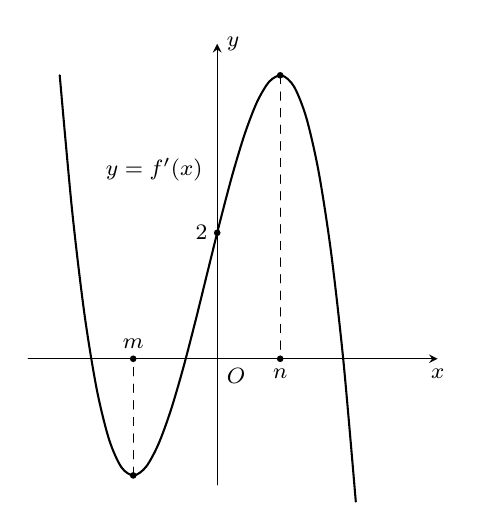
\begin{tikzpicture}[scale=0.8, font=\footnotesize, line join=round, line cap=round, >=stealth]
			\draw[->] (-3,0) --(0,0) node[below
			right]{$O$} -- (3.5,0)
			node[below]{$x$};
			\draw[->](0,-2)--(0,5)
			node[right]{$y$};
			\draw[smooth,line width=0.75]
			plot[domain=-2.5:2.2]
			(\x,{-(\x)^(3)-(1/2)*(\x)^(2)+4*\x+2});
			\draw[dashed] ({-(4/3)}, {-(50/27)}) --({-(4/3)}, 0) node[above]{$m$};
			\draw[dashed] (1, {9/2}) --(1, 0) node[below]{$n$};
			\draw (0,2) node[left]{$2$};
			\draw (-1,3) node
			{$y=f'(x)$};
			\fill ({-(4/3)}, {-(50/27)}) circle(1.5pt) 
			({-(4/3)}, 0) circle(1.5pt)
			(1, {9/2}) circle(1.5pt) 
			(1, 0) circle(1.5pt) 
			(0,2) circle(1.5pt)  
			;
		\end{tikzpicture}
	}
	
	\loigiai{
		Ta có $y'=f''\left(f(x)-2x\right) \cdot \left( f'(x)-2 \right) =0 \Leftrightarrow \hoac{&f''\left(f(x)-2x\right)=0\\& f'(x)-2 =0}\Leftrightarrow \hoac{&f(x)-2x=n \,\,(1)\\&f(x)-2x=m \,\, (2)\\& f'(x)=2. \,\, (3)}$
		\begin{itemize}
			\item  Dựa vào đồ thị $f'(x)$, ta thấy đường thẳng $y=2$ cắt đồ thị $f'(x)$ tại $3$ điểm phân biệt $x=x_1$, $x=0$, $x=x_2$. Vậy phương trình $(3)$ có $3$ nghiệm đơn.
			\item Xét hàm số $h(x)=f(x)-2x$.\\
			$h'(x)=f'(x)-2=0 \Leftrightarrow  f'(x)=2 \Leftrightarrow \hoac{&x=x_1\\&x=0\\&x=x_2.}$\\
			
\begin{tikzpicture}[>=stealth]
				\tkzTabInit[nocadre=false,lgt=1,espcl=2,deltacl=0.5]{$x$/.7 ,$y'$/.7,$y$/2}
				{$-\infty$ , $x_1$ , $0$ , $x_2$ , $+\infty$}
				\tkzTabLine{ , + , $0$ , - , $0$ , + , $0$ , - , }
				\tkzTabVar{-/$-\infty$ , +/$h(x_1)$, -/$e$ , +/$h(x_2)$ , -/$-\infty$}
			\end{tikzpicture}\\
			Dựa vào bảng biến thiên, do $e>n>m$ nên phương trình $(1)$ và $(2)$ đều có $2$ nghiệm đơn.
		\end{itemize}
		Tất cả các nghiệm của phương trình $(1)$, $(2)$, $(3)$ đều khác nhau nên hàm số đã cho có $7$ cực trị.		
	}
\end{ex}
\Closesolutionfile{ans}
%\begin{indapan}{10}
%	{ans/ans-2-GHK1-20-ChuyenHungYen-HungYen-21}
%\end{indapan}